% Created 2020-04-24 vie 23:03
% Intended LaTeX compiler: pdflatex
\documentclass[12pt,a4paper, twoside]{article} % "twoside" en lugar de "twosite"
\usepackage[utf8]{inputenc}
\usepackage{pgf-umlcd}
\usepackage{lscape}
\usepackage{tikz}
\usepackage{tikz-qtree}
\usepackage{amssymb}
\usepackage{etoolbox}
\usepackage{xparse}
\usetikzlibrary{positioning, arrows.meta, shapes}
\usepackage[T1]{fontenc}
\usepackage{graphicx}
\usepackage{apalike}
\usepackage{xcolor}
\usepackage{multirow}
\usepackage{tabularx}
\usepackage{enumitem}
\usepackage{grffile}
\usepackage{longtable}
\usepackage{wrapfig}
\usepackage{rotating}
\usepackage[normalem]{ulem}
\usepackage{amsmath}
\usepackage{textcomp}
\usepackage{capt-of}
\usepackage[spanish]{babel}
\usepackage{grffile}
%\usepackage[dvips]{epsfig}
\usepackage{listings}
\let\bibhang\relax  % Elimina la definición previa de \bibhang
\usepackage[numbers]{natbib}
\usepackage{hyperref}
\usepackage[left=2.00cm, right=2.50cm, top=2.50cm, bottom=2.00cm]{geometry}
\usepackage{fancyhdr}
\fancyhead[RO,LE]{\thepage}
\fancyhead[LO]{\emph{\uppercase{\leftmark}}}
\fancyfoot{}
\renewcommand{\headrulewidth}{1.0pt}
\pagestyle{fancy}
\date{}
\title{Circuitos lógicos programables}
\hypersetup{
    pdfauthor={},
    pdftitle={Testing de software en sistemas embebidos},
    pdfkeywords={},
    pdfsubject={},
    pdfcreator={Emacs 26.2 (Org mode 9.1.9)},
    pdflang={ spanish }
}

\linespread{1.5}

\begin{document}

\renewcommand\refname{}
\renewcommand{\contentsname}{Tabla de contenido}
\newpage

\begin{titlepage}
    \begin{center}
        \vspace*{1cm}

                
\includegraphics[width=1\textwidth]{Figuras/logoFIUBA.pdf} % Ruta al logo de FIUBA

        \vspace{1.5cm}

        \textbf{\LARGE CORDIC modo rotador}

        \vspace{4cm}
        \textbf{\Large Circuitos lógicos programables}

        \vspace{1.5cm}


        \textbf{\Large Escrito por:}\\
        \large Karen Tatiana Zamudio

        \vspace{0.8cm}

        \textbf{\Large Revisión A}\\
        \large Nicolas Álvarez

        \vfill

        \textbf{\Large Universidad de Buenos Aires}\\
        \vspace{0.2cm}

        \large  11 abril 2024

    \end{center}
\end{titlepage}
\newpage

\section*{Historial de cambios}
\label{sec:registro}

\begin{table}[ht]
  \centering
  \caption{Registro de Revisiones}
  \label{tab:registro}
  \begin{tabularx}{\linewidth}{|c|X|c|}
    \hline
    Revisión & Detalles de los cambios realizados & Fecha \\
    \hline
    0 & Creación del documento & \ 11 de abril 2024 \\
    \hline
    1 & Entrega  & \ 23 de abril 2024 \\
    \hline
  \end{tabularx}
\end{table}

\maketitle
\tableofcontents

\newpage

\section{Introducción}
\label{sec:org60390fa}

En el contexto del diseño digital y la implementación de algoritmos, el presente documento aborda la creación y análisis de un módulo de rotación basado en el algoritmo CORDIC (Coordinate Rotation Digital Computer). El algoritmo CORDIC es ampliamente utilizado en sistemas digitales para calcular funciones trigonométricas y transformaciones de coordenadas de manera eficiente.

Este documento proporcionará una visión general del diseño del módulo cordic rotator, destacando su funcionamiento, estructura interna y su implementación en una FPGA (Field-Programmable Gate Array). Además, se presentarán los resultados de simulaciones y se analizará el uso de recursos de la FPGA.


\subsection{Objetivos}
\label{subsec:org12e44a2}

Analizar y documentar el diseño, implementación y funcionamiento del módulo cordic rotator basado en el algoritmo CORDIC, así como evaluar su eficiencia y aplicabilidad en sistemas digitales.

\begin{enumerate}

\item Describir el algoritmo CORDIC y su aplicación en rotación de coordenadas: proporcionar una explicación detallada del algoritmo CORDIC y cómo se utiliza para realizar rotaciones de coordenadas cartesianas en el diseño del módulo cordic rotator.

\item Implementar el módulo cordic rotator en Verilog: crear una implementación en Verilog del módulo cordic rotator, asegurando que el código refleje correctamente la lógica del algoritmo CORDIC y que sea adecuado para su uso en sistemas digitales.

\item Realizar simulaciones del módulo y analizar su comportamiento: ejecutar simulaciones del módulo cordic rotator en un entorno de simulación, utilizando diferentes casos de prueba para evaluar su funcionamiento en una variedad de escenarios. Analizar los resultados de las simulaciones para verificar la precisión y eficacia del diseño.

\item Evaluar el uso de recursos de la FPGA: realizar un análisis exhaustivo del uso de recursos de la FPGA por parte del diseño del módulo cordic rotator, incluyendo el número de LUTs, FFs y otros recursos utilizados. Identificar áreas de mejora en términos de eficiencia y optimización del diseño.

\end{enumerate}


\subsection{Alcance}
\label{subsec:org12e44a2}

El alcance de este documento abarca la descripción detallada del diseño e implementación del módulo cordic rotator utilizando el algoritmo CORDIC en Verilog. Se incluirá una explicación exhaustiva del funcionamiento del algoritmo CORDIC y su aplicación en la rotación de coordenadas cartesianas. Además, se proporcionará el código Verilog del módulo cordic rotator junto con explicaciones detalladas de su estructura interna y su funcionamiento.

 Se realizarán simulaciones del módulo en un entorno adecuado para evaluar su comportamiento en diversos escenarios, y se analizarán los resultados obtenidos. Asimismo, se llevará a cabo un análisis del uso de recursos de la FPGA por parte del diseño, con el objetivo de evaluar su eficiencia y escalabilidad en sistemas digitales.

\newpage

\section{CORDIC}
\label{sec:orgc1c4017}

CORDIC (Coordinate Rotation Digital Computer) es un algoritmo utilizado para calcular funciones trigonométricas, como seno, coseno, arcotangente, y para realizar rotaciones y transformaciones de coordenadas de manera eficiente en sistemas digitales. Fue desarrollado en la década de 1950 por Jack E. Volder en Bell Labs.

El algoritmo CORDIC se basa en una serie de rotaciones y desplazamientos sucesivos que permiten aproximar funciones trigonométricas y realizar operaciones de rotación con un bajo costo computacional. Una de las características clave del algoritmo CORDIC es su capacidad para realizar estas operaciones utilizando únicamente operaciones de suma, resta y desplazamiento bit a bit, lo que lo hace adecuado para implementaciones en hardware digital.

El algoritmo CORDIC es especialmente útil en aplicaciones donde se requieren cálculos trigonométricos rápidos y precisos, como en sistemas de procesamiento de señales, sistemas de comunicación digital, gráficos por computadora, entre otros. Además, es altamente versátil y puede adaptarse para calcular una amplia gama de funciones trigonométricas y realizar diversas operaciones geométricas.



\subsection{CORDIC trigonométrico}
\label{sec:orgdaca22c}


El algoritmo CORDIC (Coordinate Rotation Digital Computer) Trigonométrico es un método iterativo utilizado para calcular funciones trigonométricas como el seno ($\sin$), coseno ($\cos$), arcoseno ($\arcsin$) y arcocoseno ($\arccos$). Funciona mediante iteraciones de rotación y desplazamiento, donde cada iteración aproxima gradualmente el valor deseado de la función trigonométrica. El algoritmo se basa en la representación de un ángulo en coordenadas cartesianas $(X, Y)$ y utiliza rotaciones sucesivas para acercarse al ángulo objetivo. A medida que las iteraciones continúan, el valor de salida converge hacia el valor correcto con una precisión determinada.

En cada iteración del algoritmo CORDIC Trigonométrico, se realiza una rotación y un desplazamiento de las coordenadas $(X, Y)$. La rotación se realiza mediante el ajuste de los ángulos de las coordenadas, lo que permite acercarse al ángulo objetivo. El desplazamiento se utiliza para ajustar las magnitudes de las coordenadas y garantizar que la convergencia del algoritmo sea adecuada. Estas iteraciones se repiten hasta que se alcanza la precisión deseada en el cálculo de la función trigonométrica.

Por ejemplo, para calcular el seno de un ángulo dado utilizando el algoritmo CORDIC Trigonométrico, se inicializan las coordenadas $(X, Y)$ con valores apropiados y se realizan iteraciones de rotación y desplazamiento hasta que se alcanza la precisión deseada. El valor de $Y$ al final de las iteraciones representa el valor aproximado del seno del ángulo dado. De manera similar, se pueden calcular el coseno, el arcoseno y el arcocoseno utilizando adaptaciones del algoritmo CORDIC Trigonométrico.



La precisión y la convergencia del algoritmo CORDIC Trigonométrico dependen del número de iteraciones realizadas y del número de bits utilizados para representar los valores de las coordenadas. En general, el algoritmo converge rápidamente y proporciona resultados precisos con un número suficiente de iteraciones. Sin embargo, la precisión puede verse afectada por la representación finita de los números en sistemas digitales y por la resolución de las operaciones de rotación y desplazamiento.

El algoritmo CORDIC trigonométrico se utiliza en una amplia gama de aplicaciones en sistemas digitales, incluyendo procesamiento de señales, comunicaciones, gráficos por computadora, sistemas de navegación y más. Se utiliza para calcular funciones trigonométricas de manera eficiente y precisa en sistemas donde se requieren cálculos frecuentes de ángulos y funciones trigonométricas. Su implementación en hardware digital es especialmente adecuada debido a su simplicidad y eficiencia en términos de recursos computacionales.

Las ecuaciones para las iteraciones de rotación y desplazamiento en el algoritmo CORDIC Trigonométrico pueden ser expresadas como:

\begin{equation}
    \begin{aligned}
        X_{i+1} &= X_i - \delta_i \cdot Y_i \cdot 2^{-i}, \\
        Y_{i+1} &= Y_i + \delta_i \cdot X_i \cdot 2^{-i}, \\
        Z_{i+1} &= Z_i - \delta_i \cdot \text{atanh}(2^{-i}),
    \end{aligned}
\end{equation}

donde $i$ es el índice de iteración, $\delta_i$ es el signo de la rotación en la iteración $i$, $X_i$, $Y_i$ son las coordenadas en la iteración $i$, y $Z_i$ es el ángulo acumulado hasta la iteración $i$.  



\subsection{CORDIC vectorial}
\label{sec:orgdaca22c}


El algoritmo CORDIC Vectorial utiliza un enfoque similar al CORDIC Trigonométrico, pero se enfoca en manipular vectores en lugar de solo ángulos. Permite realizar rotaciones y transformaciones de coordenadas en sistemas de coordenadas cartesianas o polares de manera eficiente. 

En un sistema de coordenadas cartesianas, las operaciones del CORDIC Vectorial pueden utilizarse para rotar un vector en el plano XY. Por otro lado, en un sistema de coordenadas polares, el algoritmo puede utilizarse para convertir coordenadas cartesianas a polares y viceversa, así como para realizar rotaciones de vectores en el plano radial.

La eficiencia y precisión del CORDIC Vectorial lo hacen adecuado para una variedad de aplicaciones en sistemas digitales, como procesamiento de señales, modulación y demodulación en sistemas de comunicaciones, y transformaciones geométricas en gráficos por computadora. Además, su estructura iterativa permite su implementación eficiente en hardware digital, lo que lo convierte en una opción popular en sistemas embebidos y sistemas de tiempo real donde los recursos son limitados.


\subsection{CORDIC logarítmico}
\label{sec:orgdaca22c}

El algoritmo CORDIC logarítmico utiliza una serie de iteraciones para aproximar funciones logarítmicas y exponenciales, así como operaciones relacionadas como la raíz cuadrada y el exponente. A través de un proceso iterativo, el algoritmo calcula las aproximaciones de estas funciones con una precisión deseada.

Una de las características clave del CORDIC logarítmico es su capacidad para calcular estas funciones de manera eficiente y precisa utilizando un enfoque iterativo y estructuras de datos simples. Esto lo hace adecuado para su implementación en sistemas digitales donde se requieren cálculos de funciones no trigonométricas con recursos limitados.

El CORDIC logarítmico tiene una amplia gama de aplicaciones en sistemas digitales, incluyendo procesamiento de señales, compresión de datos, criptografía y más. Se utiliza en situaciones donde se requiere el cálculo rápido y preciso de funciones logarítmicas y exponenciales, así como operaciones relacionadas como la raíz cuadrada y el exponente. Su eficiencia y precisión lo hacen valioso en una variedad de aplicaciones de sistemas digitales.


\newpage

\section{Implementación CORDIC rotator}
\label{sec:orgc1c4017}

En esta sección, se detalla la implementación del módulo CORDIC Rotator en Verilog. El módulo CORDIC Rotator es una implementación hardware del algoritmo CORDIC (Coordinate Rotation Digital Computer), diseñado para realizar rotaciones de vectores en el plano cartesiano. El algoritmo CORDIC se utiliza ampliamente en sistemas digitales para calcular funciones trigonométricas, transformaciones de coordenadas y otras operaciones matemáticas de manera eficiente. En esta sección, se explicará paso a paso la implementación del módulo CORDIC rotator, incluyendo la configuración de parámetros, la definición de la tabla de arco tangente, las iteraciones del algoritmo y la salida del módulo. Cada parte de la implementación se analizará en detalle, acompañada de su correspondiente código en Verilog.

\subsection{Configuración de Tiempo y Declaración de Módulo}

El código comienza con la configuración del \texttt{timescale} y la definición de parámetros utilizados en el módulo. El parámetro \texttt{c parameter} determina el ancho de bits de los datos de entrada y salida, mientras que \texttt{STG} se utiliza para definir el ancho de bits de los vectores \texttt{X} e \texttt{Y}. Luego, se declara el módulo \texttt{cordic rotator} con sus entradas (\texttt{clock}, \texttt{angle}, \texttt{Xin}, \texttt{Yin}) y salidas (\texttt{Xout}, \texttt{Yout}).

\begin{lstlisting}[language=Verilog]
`timescale 1ns/100ps

module cordic_rotator (
    input clock,
    input signed [31:0] angle,
    input signed [c_parameter - 1:0] Xin,
    input signed [c_parameter - 1:0] Yin,
    output signed [c_parameter:0] Xout,
    output signed [c_parameter:0] Yout
);

parameter c_parameter = 16;
localparam STG = c_parameter;
\end{lstlisting}

\subsection{Declaración de la Tabla \texttt{atan\_table}}

La tabla \texttt{atan\_table} contiene los valores de la función arco tangente utilizados en el algoritmo CORDIC. Estos valores están precalculados y se utilizan para realizar las operaciones de rotación en el módulo. La tabla está definida como un arreglo de 31 bits con 31 entradas, cada una representando un ángulo específico.

\begin{lstlisting}[language=Verilog]

wire signed [31:0] atan_table [0:30];
assign atan_table[00] = 32'b00100000000000000000000000000000; 
// Resto de asignaciones de la tabla atan_table...

\end{lstlisting}

\subsection{Inicialización de registros y asignación de cuadrante}

Se inicializan los registros \texttt{X}, \texttt{Y} y \texttt{Z}, que se utilizan para almacenar los datos en cada etapa del algoritmo CORDIC. Luego, se calcula el cuadrante en el que se encuentra el ángulo de rotación para determinar cómo se deben tratar los datos de entrada.

\subsubsection{Cuadrante I}

En el cuadrante I, el ángulo de rotación se encuentra en el rango de 0 a $\pi$/2. En este caso, no es necesario realizar ninguna modificación en los datos de entrada, ya que están en el rango adecuado para ser procesados por el algoritmo CORDIC. Por lo tanto, los valores de las coordenadas X e Y del vector de entrada (\texttt{Xin} y \texttt{Yin}) se asignan directamente a los registros \texttt{X[0]} y \texttt{Y[0]}, respectivamente. Además, el ángulo de rotación (\texttt{angle}) se asigna directamente al registro \texttt{Z[0]}.

\begin{lstlisting}[language=Verilog]
       case (quadrant)
           2'b00: begin // Cuadrante I
               X[0] <=   Xin;
               Y[0] <=   Yin;
               Z[0] <=   angle;
\end{lstlisting}

Este caso se activa cuando los bits de signo del ángulo son 0, indicando que el ángulo se encuentra en el primer cuadrante.

\subsubsection{Cuadrante II}

En el cuadrante II, el ángulo de rotación se encuentra en el rango de $\pi$/2 a $\pi$. Para ajustar los datos de entrada al rango adecuado para el algoritmo CORDIC, se realiza una pre-rotación del ángulo. En este caso, el ángulo se resta de $\pi$ para asegurar que esté dentro del rango de -$\pi$/2 a 0. Los valores de las coordenadas X e Y del vector de entrada se asignan a los registros \texttt{X[0]} y \texttt{Y[0]}, respectivamente, de la misma manera que en el cuadrante I.

\begin{lstlisting}[language=Verilog]
       2'b01: begin // Cuadrante II
               X[0] <=    Xin;
               Y[0] <=    Yin;
               Z[0] <=  32'b10000000000000000000000000000000 - angle;                  
\end{lstlisting}

Este caso se activa cuando el bit de signo más significativo del ángulo es 0 y el siguiente bit es 1, indicando que el ángulo se encuentra en el segundo cuadrante.

\subsubsection{Cuadrante III}

En el cuadrante III, el ángulo de rotación se encuentra en el rango de -$\pi$ a -$\pi$/2. Al igual que en el cuadrante II, se realiza una pre-rotación del ángulo restando $\pi$ para asegurar que esté dentro del rango de -$\pi$/2 a 0. Los valores de las coordenadas X e Y del vector de entrada se asignan a los registros \texttt{X[0]} y \texttt{Y[0]}, respectivamente, de la misma manera que en los cuadrantes I y II.

\begin{lstlisting}[language=Verilog]
       2'b10: begin // Cuadrante III
               X[0] <=    Xin;
               Y[0] <=    Yin;
               Z[0] <=    angle - 32'b10000000000000000000000000000000; 
\end{lstlisting}

Este caso se activa cuando el bit de signo más significativo del ángulo es 1 y el siguiente bit es 0, indicando que el ángulo se encuentra en el tercer cuadrante.

\subsubsection{Cuadrante IV}

En el cuadrante IV, el ángulo de rotación se encuentra en el rango de -$\pi$/2 a 0. Para ajustar los datos de entrada al rango adecuado para el algoritmo CORDIC, se realiza una pre-rotación del ángulo restando 2$\pi$ para asegurar que esté dentro del rango de -$\pi$/2 a -$\pi$. Los valores de las coordenadas X e Y del vector de entrada se asignan a los registros \texttt{X[0]} y \texttt{Y[0]}, respectivamente, de la misma manera que en los cuadrantes I, II y III.


\begin{lstlisting}[language=Verilog]
       2'b10: begin // Cuadrante III
               X[0] <=    Xin;
               Y[0] <=    Yin;
               Z[0] <=    angle - 32'b10000000000000000000000000000000; 
\end{lstlisting}

Este caso se activa cuando los bits de signo del ángulo son 1, indicando que el ángulo se encuentra en el cuarto cuadrante.



\subsection{Banco de pruebas}

El banco de pruebas proporcionado se encarga de simular el módulo \texttt{cordic\_rotator} y generar formas de onda de entrada para probar su funcionalidad. Aquí tienes una explicación detallada de su funcionamiento:

\subsubsection{Parámetros y variables locales}
Se definen algunos parámetros y variables locales para el tamaño de los datos de entrada (\texttt{SZ}), los valores booleanos (\texttt{FALSE} y \texttt{TRUE}), y el valor de la señal de entrada (\texttt{VALUE}), que se reduce para ajustarse a la ganancia del sistema.

\begin{lstlisting}[language=Verilog]

localparam SZ = 16; 

reg [SZ-1:0] Xin, Yin;
reg [31:0] angle;
wire [SZ:0] Xout, Yout;
reg CLK_100MHZ;

localparam FALSE = 1'b0;
localparam TRUE = 1'b1;

// reducido por un factor de 1.647 ya que es la ganancia del sistema (k)
localparam VALUE = 32000/1.647; 

\end{lstlisting}

\subsubsection{Inicialización}
Antes de comenzar la simulación, se inicializan las variables y las señales de entrada. Se establece \texttt{start} en \texttt{FALSE}, se inicializa la señal de reloj \texttt{CLK\_100MHZ}, el ángulo en cero, y se establece un valor inicial para \texttt{Xin} y \texttt{Yin}.

\begin{lstlisting}[language=Verilog]
initial
begin
    start = FALSE;
    CLK_100MHZ = 1'b0;
    angle = 0;
    Xin = VALUE;
    Yin = 1'd0;
    i = 0;
  
    #1000;
    @(posedge CLK_100MHZ);
    start = TRUE;
\end{lstlisting}

\subsubsection{Generación de formas de onda}
Durante la simulación, se genera una señal de reloj de 100 MHz (\texttt{CLK\_100MHZ}). Después de un breve período de espera, se activa \texttt{start} para indicar que la simulación comienza y se comienza a generar una secuencia de ángulos para probar el módulo \texttt{cordic\_rotator}.

\begin{lstlisting}[language=Verilog]
for (i = 0; i < 360; i = i + 1)  

begin
    @(posedge CLK_100MHZ);
    #11700
    start = FALSE;
    angle = ((1 << 32)*(i+1))/360;
end
\end{lstlisting}

\subsubsection{Generación del reloj}
Se genera una señal de reloj de 100 MHz (\texttt{CLK\_100MHZ}) con una duración de tiempo determinada por \texttt{CLK100\_SPEED}.

\begin{lstlisting}[language=Verilog]
parameter CLK100_SPEED = 10; // 100Mhz = 10nS

initial
begin
    CLK_100MHZ = 1'b0;
    $display("CLK_100MHZ iniciado");
    #5;
    forever
    begin
        #(CLK100_SPEED/2) CLK_100MHZ = 1'b1;
        #(CLK100_SPEED/2) CLK_100MHZ = 1'b0;
    end
end
\end{lstlisting}


\subsubsection{Salida del módulo}

Finalmente, se asignan las salidas \texttt{Xout} y \texttt{Yout} del módulo con los valores calculados después de completar todas las iteraciones del algoritmo CORDIC. Estas salidas representan las coordenadas rotadas del vector de entrada.

\begin{lstlisting}[language=Verilog]

        assign Xout = X[STG - 1];
        assign Yout = Y[STG - 1];

\end{lstlisting}



\subsection{Simulación}
\label{sec:orgdaca22c}


En este documento, se describe el proceso para realizar la simulación del diseño en Vivado y posteriormente generar el archivo .bit que se utilizará para la programación de la FPGA.

\subsection{Simulación en vivado}

Para realizar la simulación en Vivado, sigue estos pasos:

\begin{enumerate}
    \item \textbf{Crear un proyecto:} Abre Vivado y crea un nuevo proyecto. Selecciona la opción de crear un diseño de tipo "RTL Project" e importa los archivos fuente de tu diseño, incluyendo el código Verilog o VHDL del rotador CORDIC.

    \begin{figure}[ht]
    \centering
    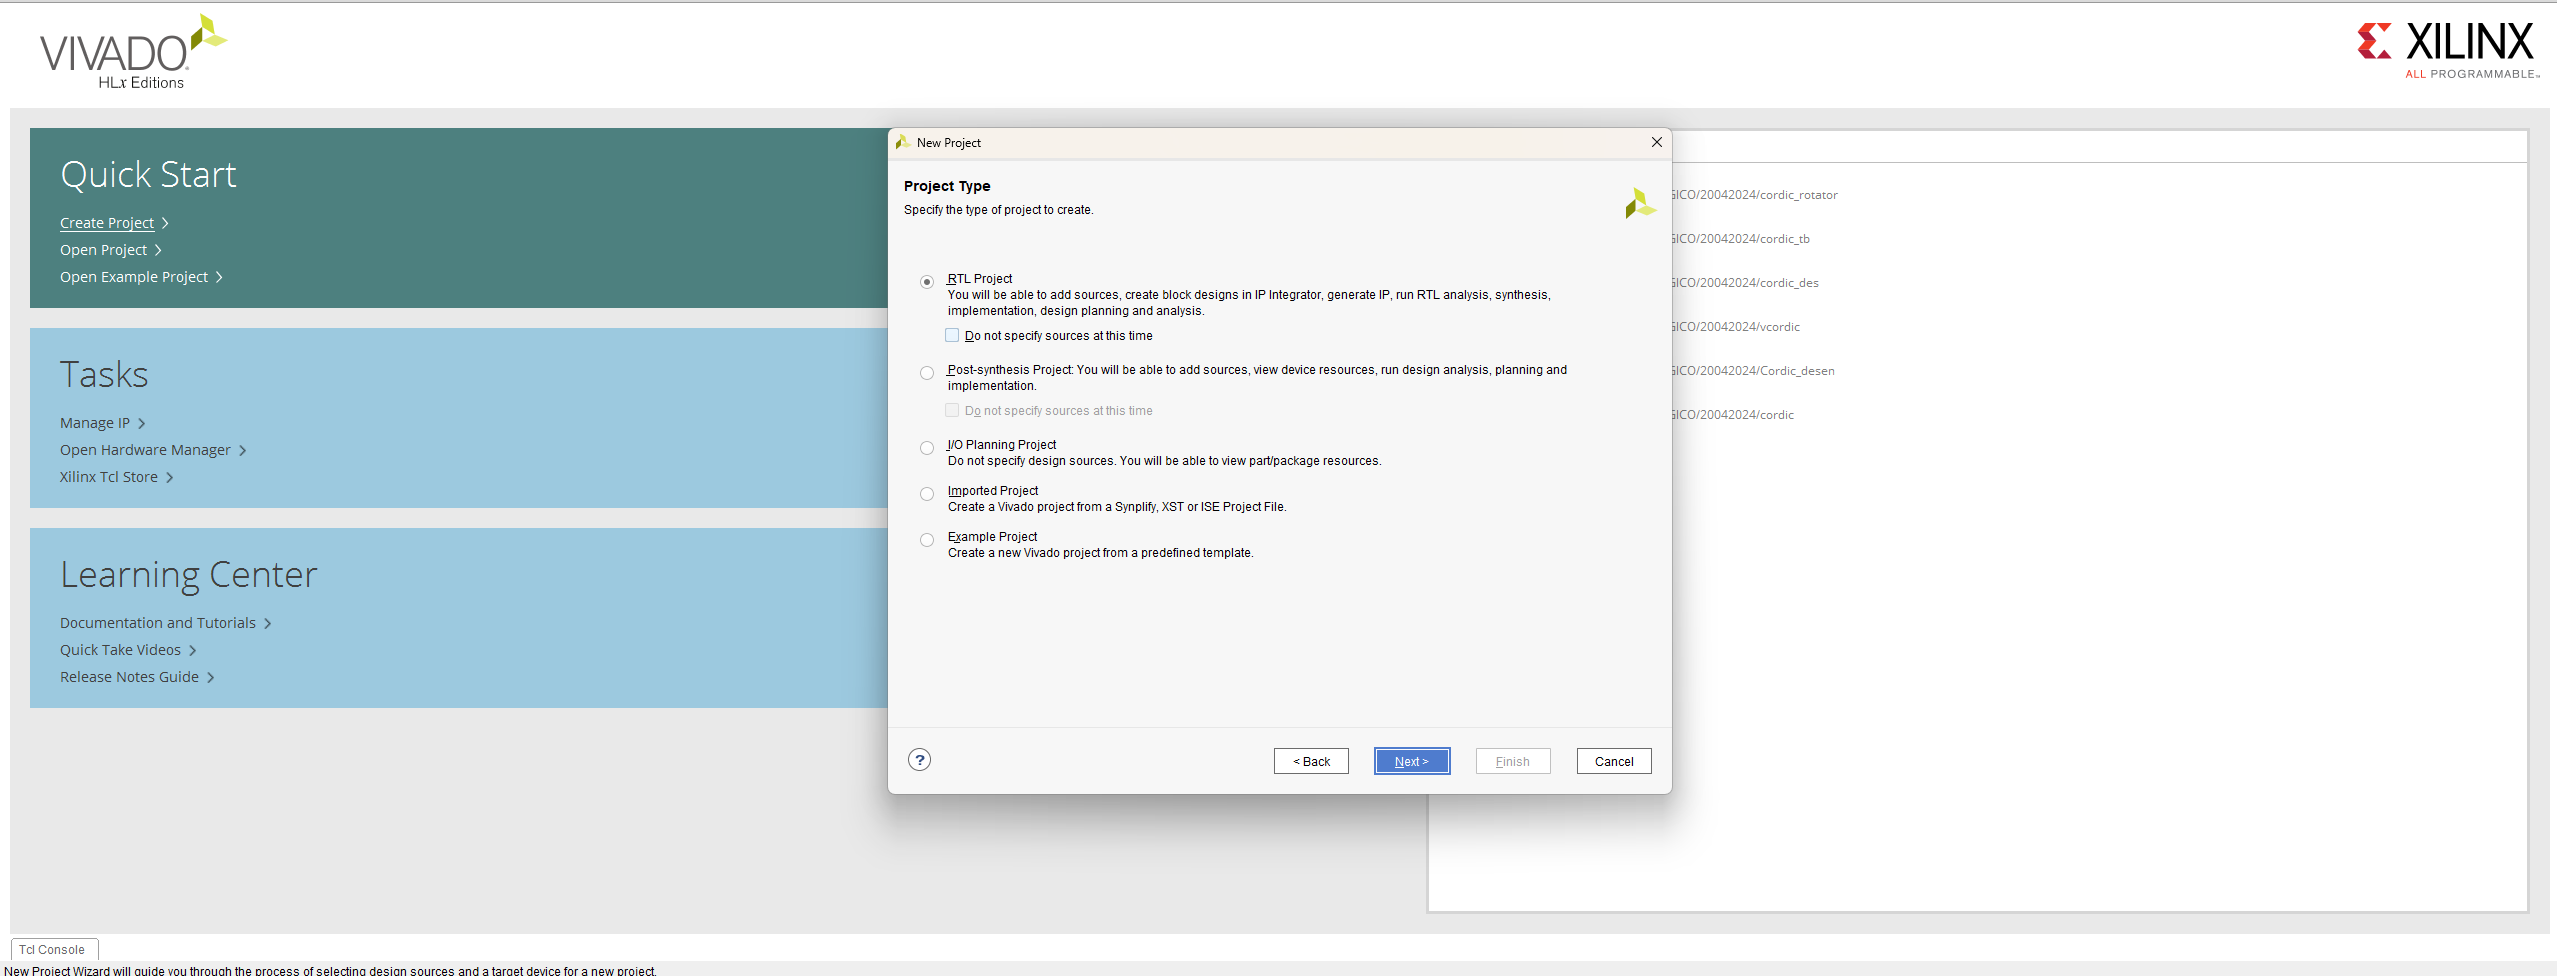
\includegraphics[width=0.8\textwidth]{./Figuras/New_project.png}
    \caption{Crear nuevo proyecto en Vivado}
    \label{fig:new_proyect}
    \end{figure}
    
        
    \begin{figure}[ht]
    \centering
    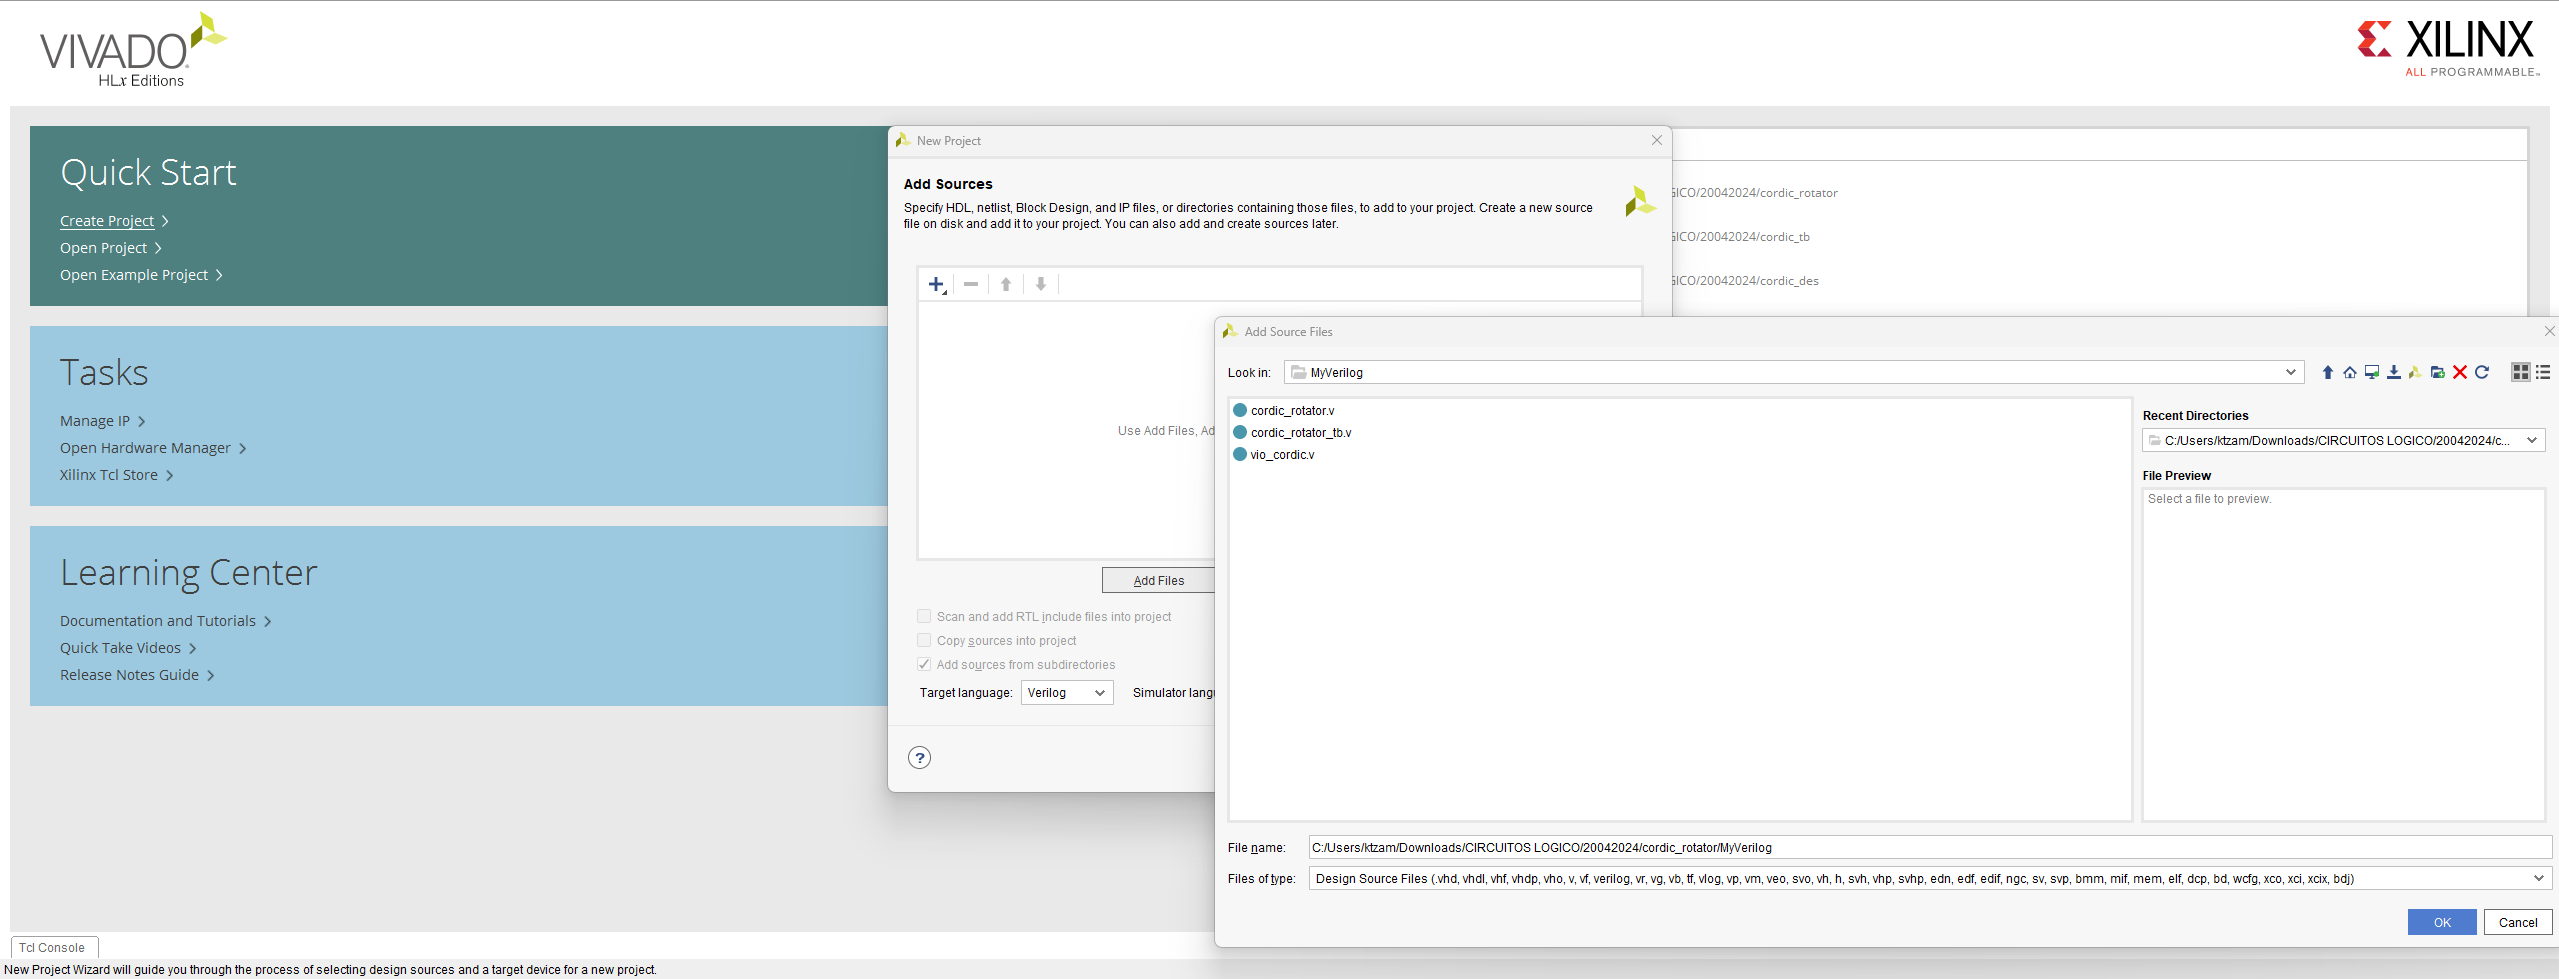
\includegraphics[width=0.8\textwidth]{./Figuras/add_source.png}
    \caption{Importacion de archivos fuente}
    \label{fig:add_source}
    \end{figure} 
       
   
    
    \item \textbf{Configurar simulación:} una vez que hayas creado el proyecto. Ve a la pestaña "Flow Navigator" y selecciona "Simulation". Aquí puedes configurar las opciones de simulación, como el tipo de simulador a utilizar y los archivos de simulación a incluir.

    
    \item \textbf{Ejecutar la simulación:} después de configurar la simulación, ejecútala haciendo clic en el botón "Run Simulation". Vivado ejecutará la simulación y generará resultados que podrás analizar.
    \begin{figure}[ht]
    \centering
    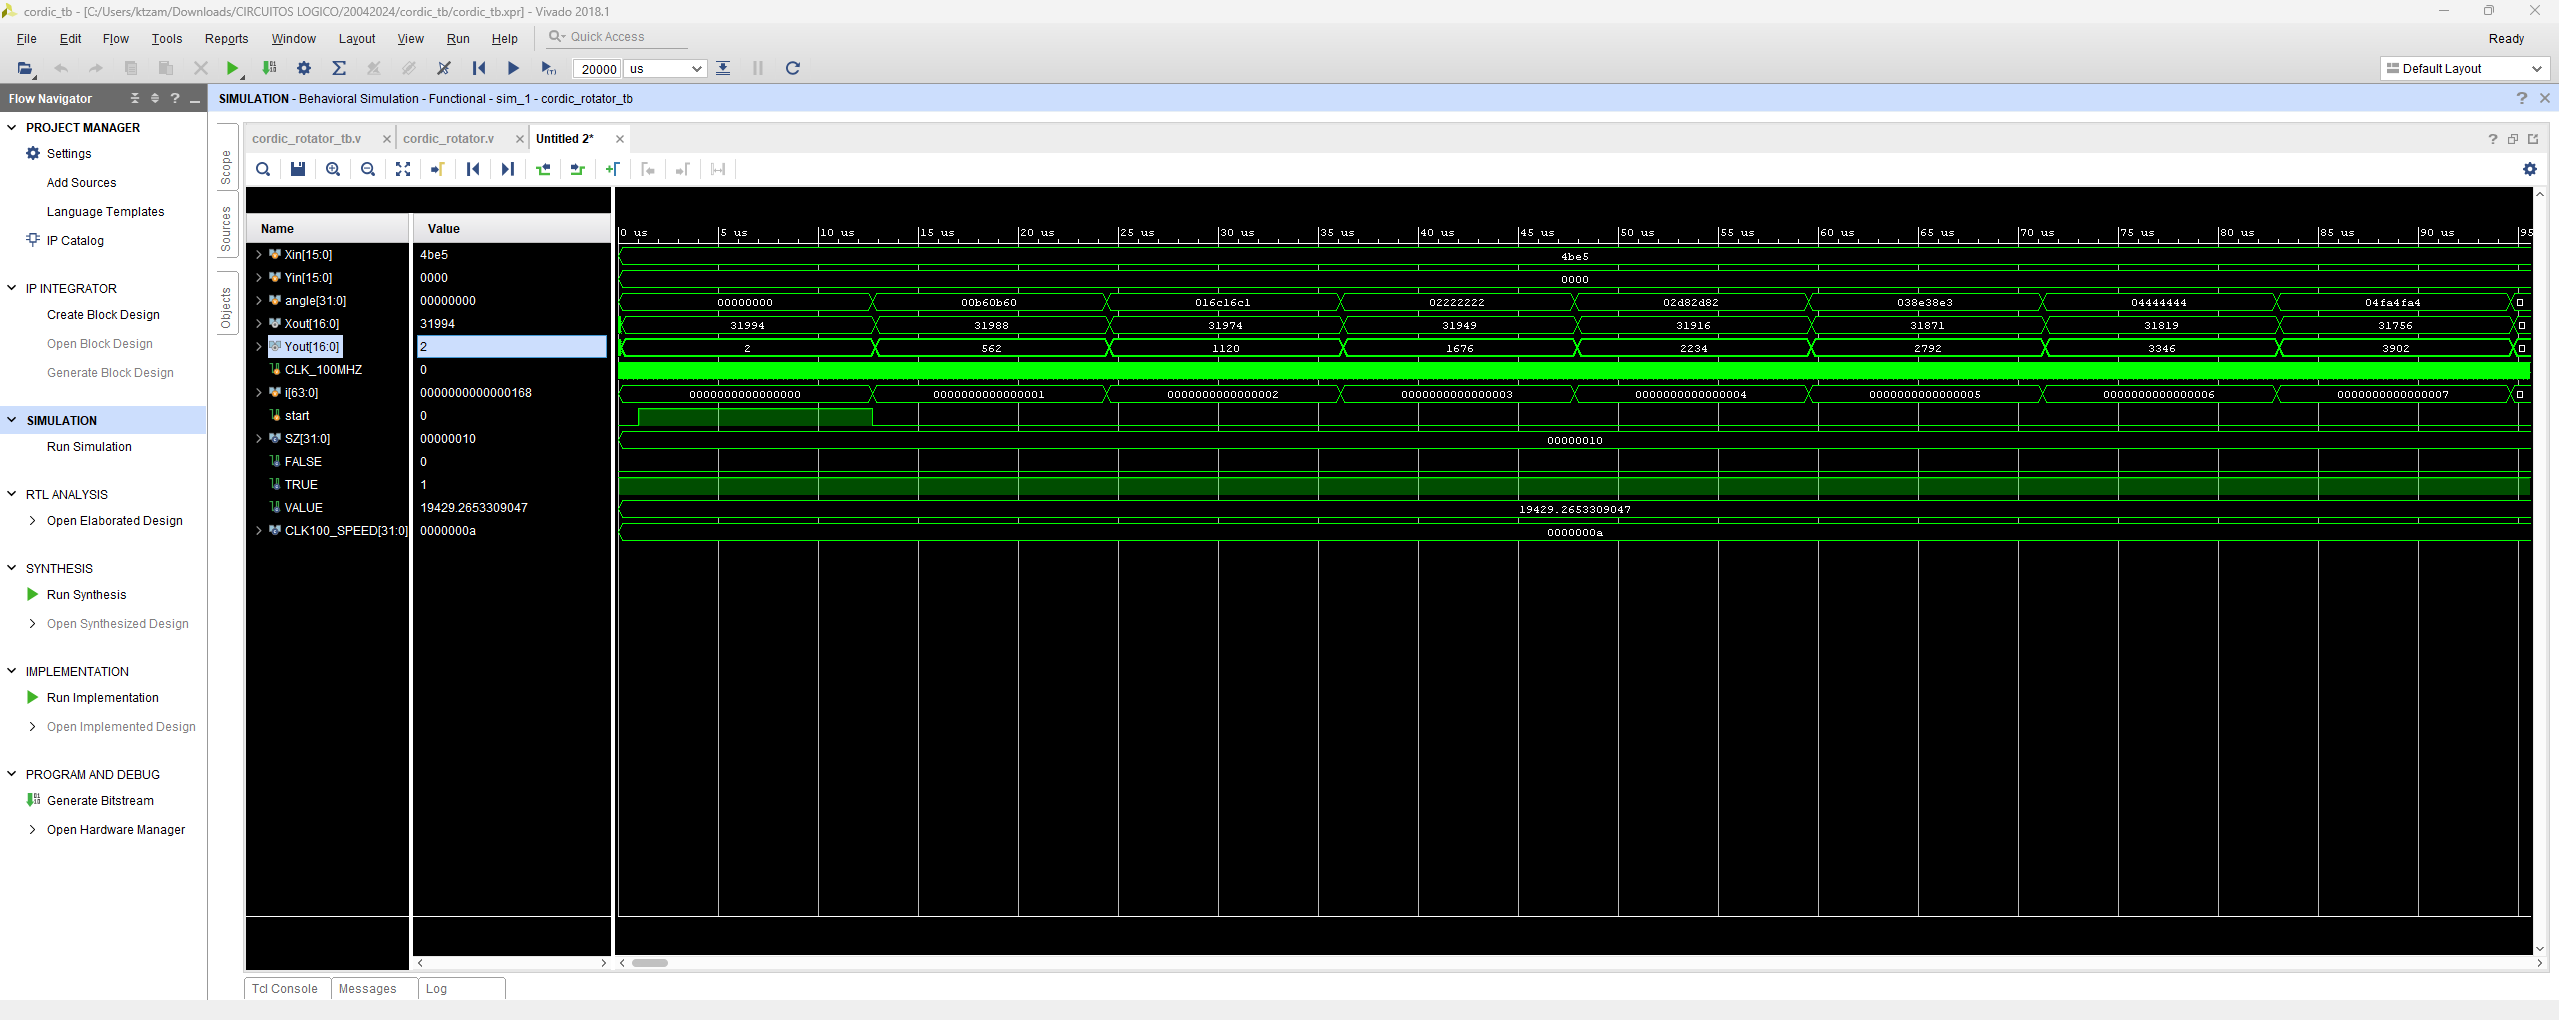
\includegraphics[width=0.8\textwidth]{./Figuras/Run_simulacion_visual.png}
    \caption{simulación en Vivado}
    \label{fig:simulación}
    \end{figure}
    
   
        \item \textbf{Análisis de resultados:} una vez completada la simulación, analiza los resultados en Vivado. Puedes revisar las formas de onda de las señales de entrada y salida, así como cualquier mensaje de advertencia o error que pueda haberse generado durante la simulación.
\end{enumerate}


    \begin{figure}[ht]
    \centering
    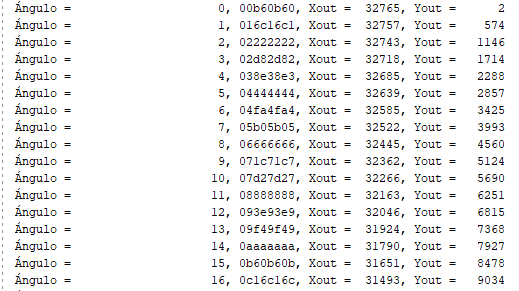
\includegraphics[width=0.6\textwidth]{./Figuras/Resultado.png}
    \caption{Resultados obtenidos de la simulación}
    \label{fig:esquema}
    \end{figure}

    

\subsection{Uso de la IP VIO en el módulo \texttt{cordic\_rotator}}

El uso de la IP VIO (Virtual Input/Output) en este contexto proporciona una herramienta poderosa para la simulación y depuración del algoritmo CORDIC implementado en el módulo \texttt{cordic\_rotator}. La IP VIO es una característica de las herramientas de diseño de FPGA, como Xilinx Vivado, que permite la visualización y manipulación de señales dentro de un diseño durante la simulación.

Las entradas de la IP VIO están conectadas a las salidas del módulo \texttt{cordic\_rotator}, mientras que las salidas de la IP VIO se conectan a las entradas del mismo módulo. Esto permite inyectar señales controladas y observar las salidas correspondientes del algoritmo CORDIC en tiempo real durante la simulación.


Al conectar las salidas del \texttt{cordic\_rotator} a las entradas de la IP VIO y viceversa, puedes controlar las condiciones de entrada del algoritmo CORDIC y observar las respuestas resultantes. Esto es especialmente útil para verificar el comportamiento del algoritmo bajo diferentes condiciones de entrada y para depurar posibles problemas en la lógica de diseño.


    \begin{figure}[ht]
    \centering
    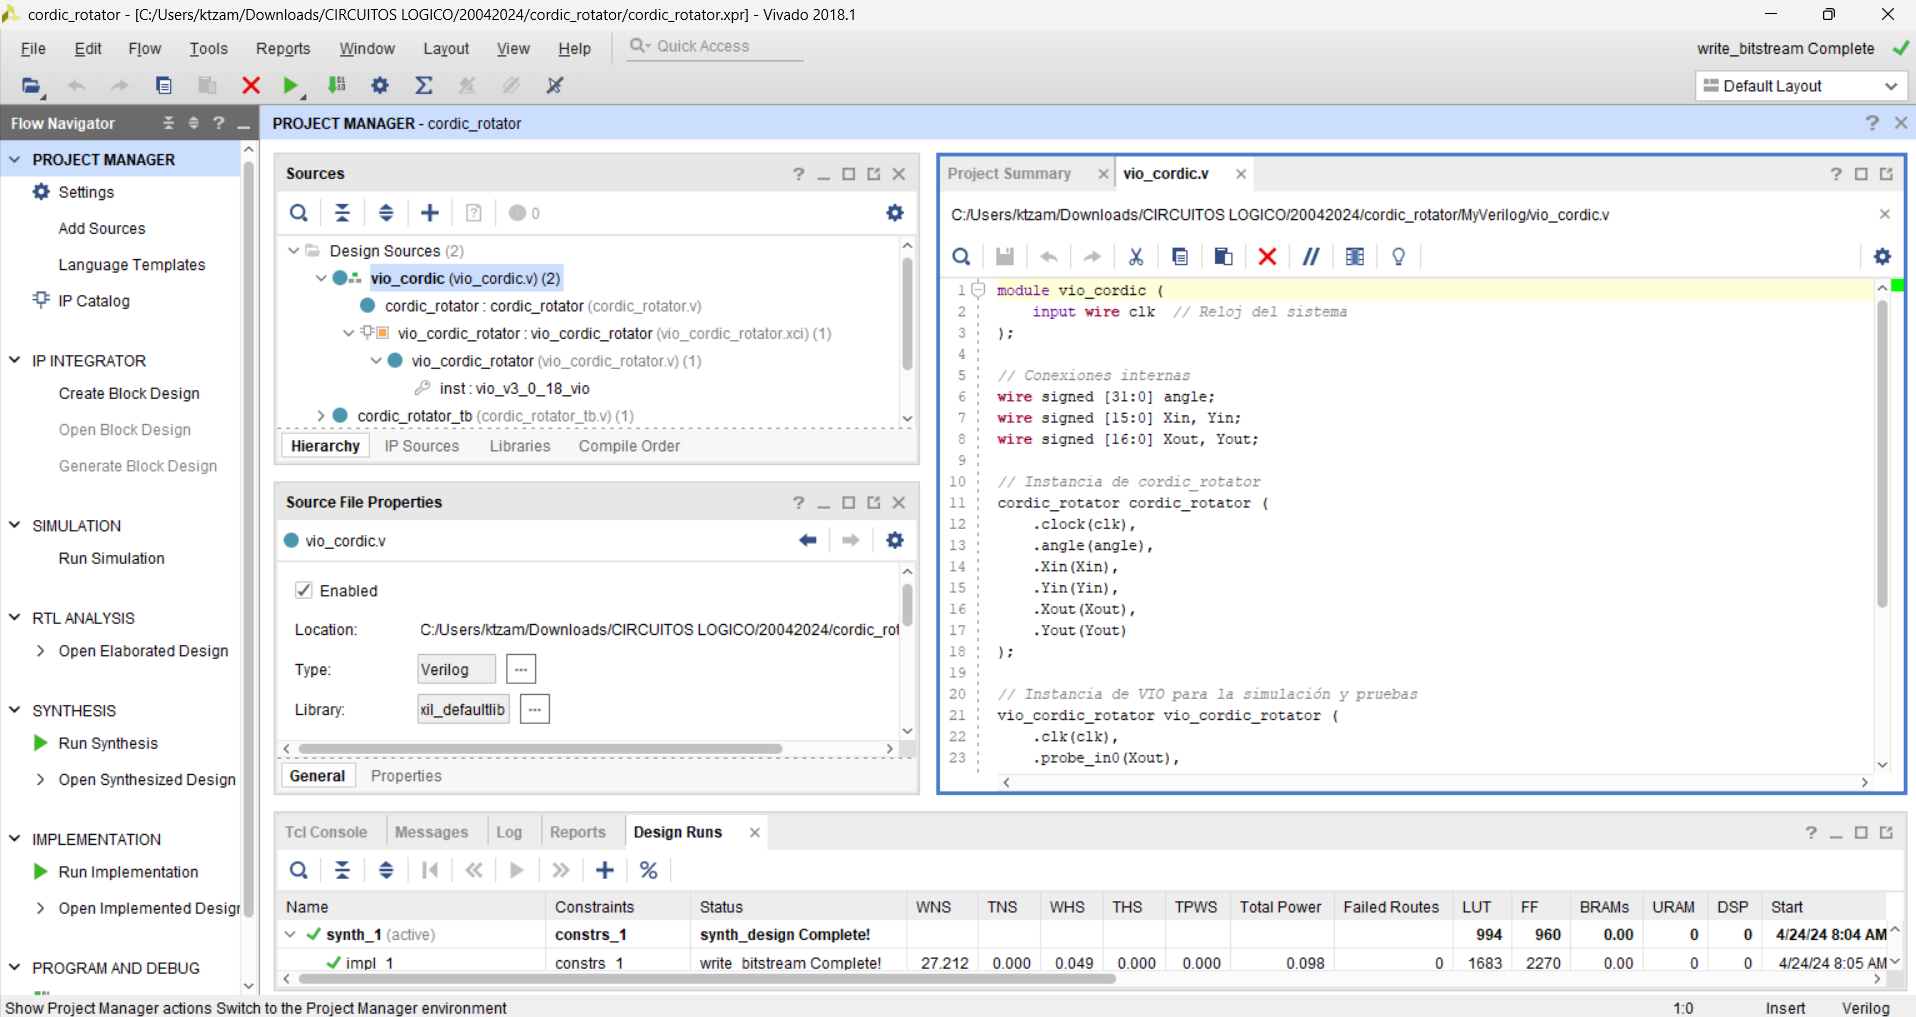
\includegraphics[width=0.8\textwidth]{./Figuras/IP_VIO.png}
    \caption{IP VIO}
    \label{fig:ip_vio}
    \end{figure}



En resumen, la IP VIO se utiliza en este contexto para proporcionar una interfaz gráfica que permite inyectar señales de entrada y observar las salidas correspondientes del algoritmo CORDIC durante la simulación. Esto facilita la depuración y validación del diseño, mejorando así la eficiencia y la precisión del algoritmo implementado.


\subsection{Esquema}

El esquema utilizado para conectar las entradas y salidas del rotador CORDIC durante la simulación en Vivado se muestra en la Figura \ref{fig:esquema}.

\begin{figure}[ht]
    \centering
    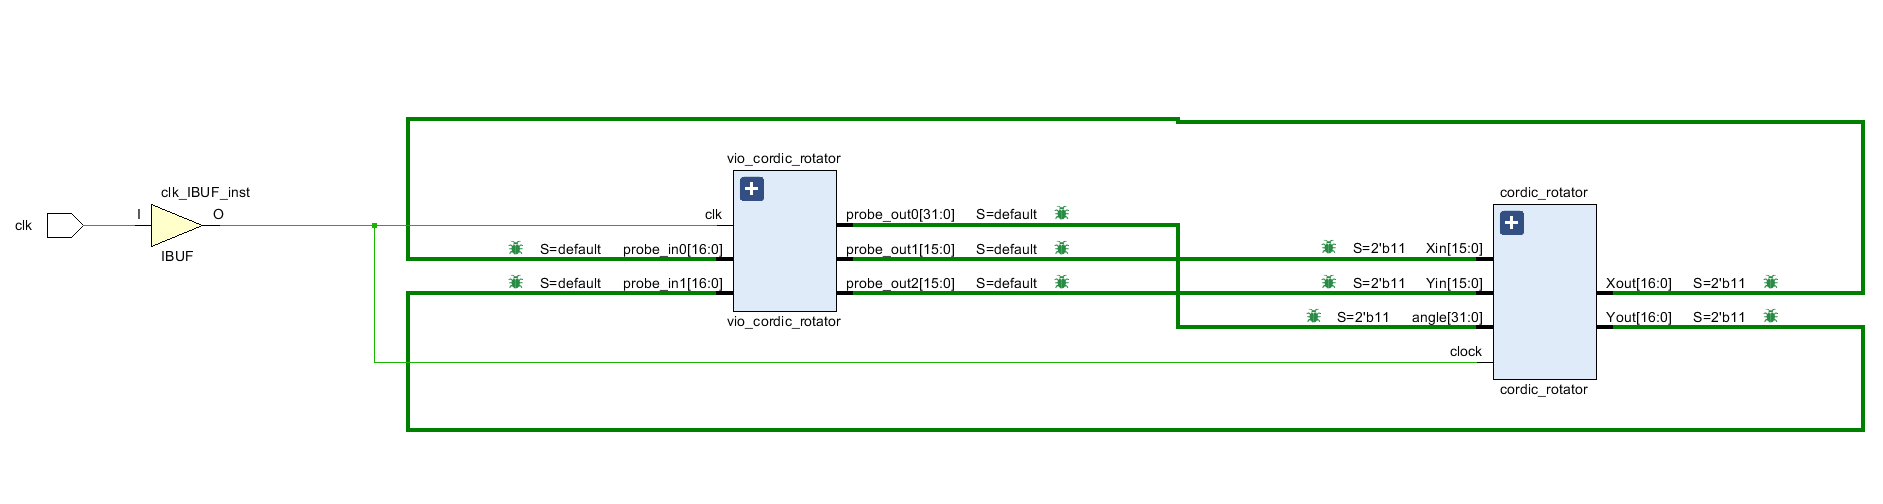
\includegraphics[width=1\textwidth]{./Figuras/schematic.png}
    \caption{Esquema utilizado para la simulación en Vivado IP VIO y CORDIC}
    \label{fig:esquema}
\end{figure}

    
    
    \begin{figure}[ht]
    \centering
    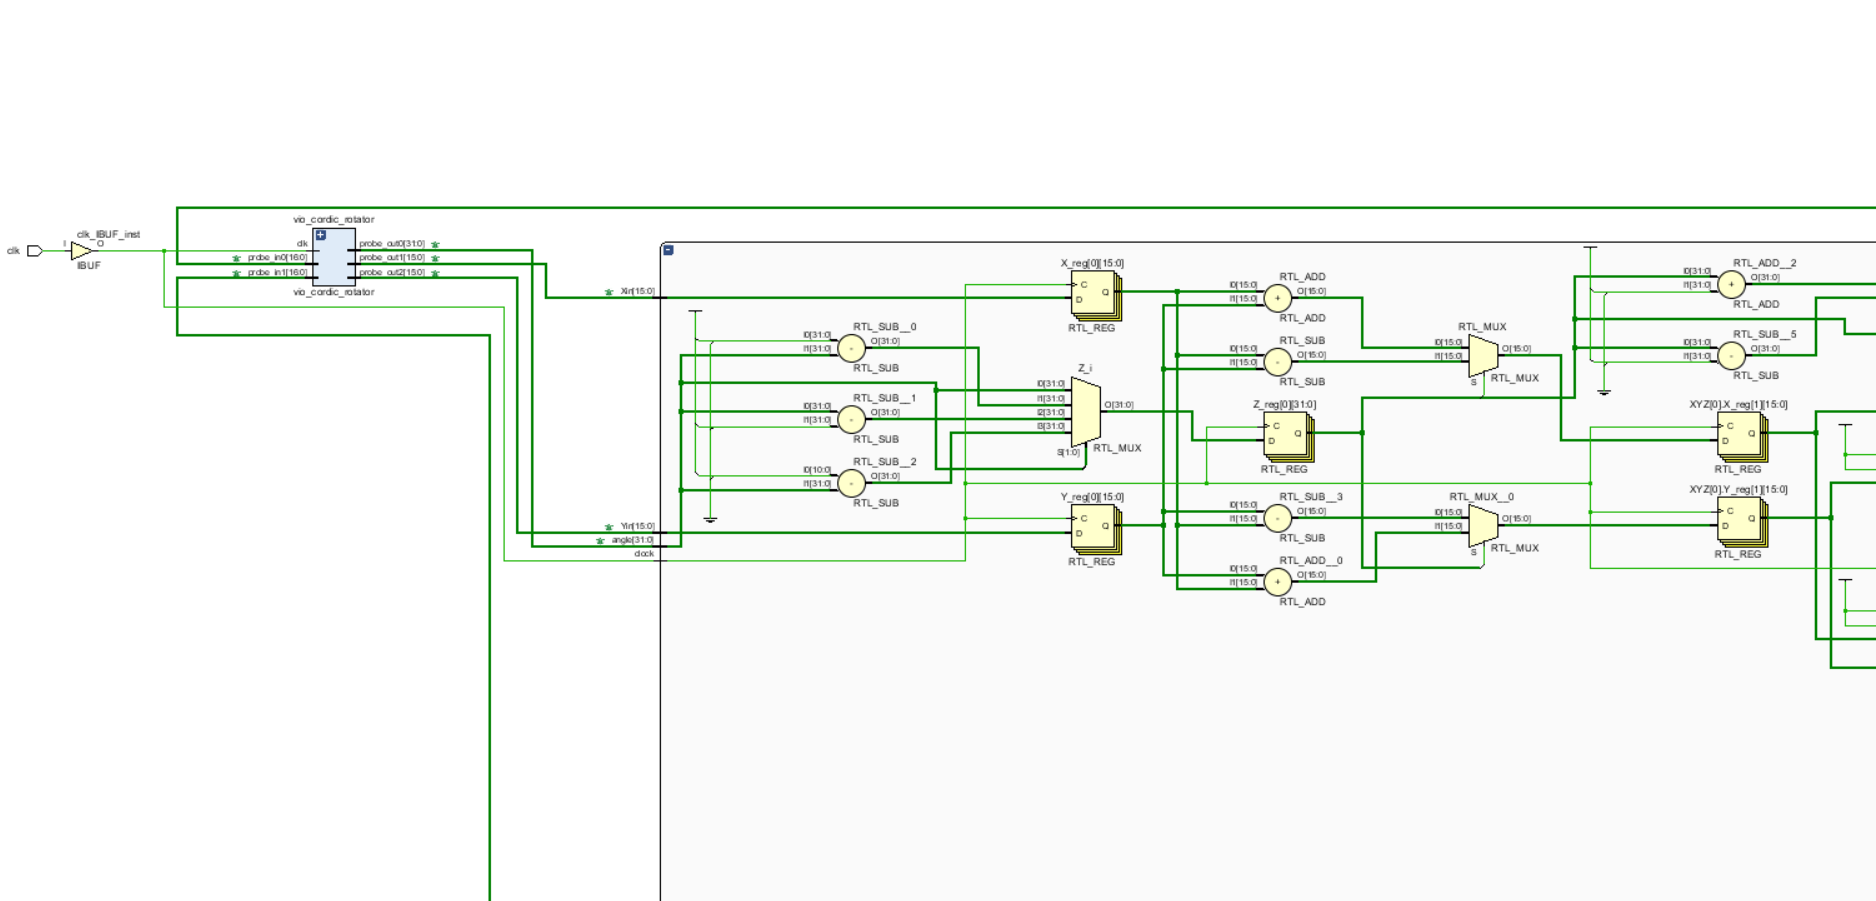
\includegraphics[width=1\textwidth]{./Figuras/squematic_cordic.png}
    \caption{Esquema de CORDIC}
    \label{fig:esquema}
\end{figure}


\subsection{Generación del archivo .bit}

Una vez completado y verificado la simulación en vivado, es posible generar generar el archivo .bit para programar la FPGA. A traves de los siguientes pasos:

\begin{enumerate}
    \item \textbf{Implementación del diseño:} en Vivado, en la pestaña "Flow Navigator" y selecciona "Implementation". Aquí,  se ejecuta el proceso de implementación para sintetizar y asignar el diseño a los recursos de la FPGA.
    
    \item \textbf{Generación del Bitstream:} después de completar la implementación, en la pestaña "Generate Bitstream" en Vivado. Se ejecuta este proceso para generar el archivo .bit, que contiene la configuración del diseño para la FPGA.
    
    \begin{figure}[ht]
    \centering
    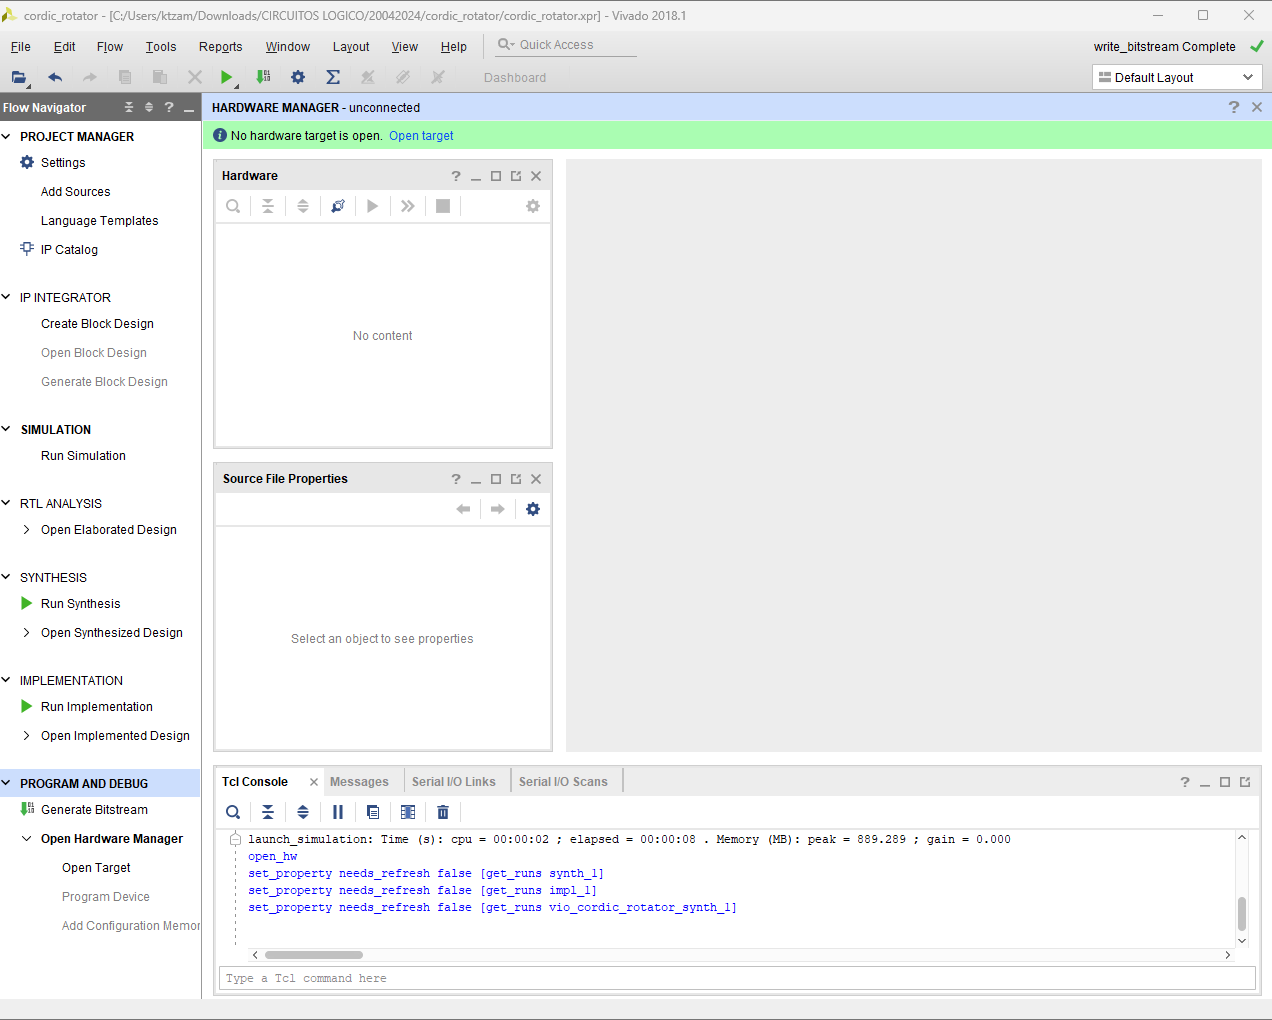
\includegraphics[width=0.65\textwidth]{./Figuras/bitsteam_complete.png}
    \caption{bitsteam completo}
    \label{fig:bitsteam_complete}
\end{figure}

    
    \item \textbf{Programación de la FPGA:} una vez generado el archivo .bit, se utiliza para programar la FPGA. Conecta la FPGA a tu computadora y utiliza el software de programación de Vivado para cargar el archivo .bit en la FPGA.
\end{enumerate}

    \begin{figure}[ht]
    \centering
    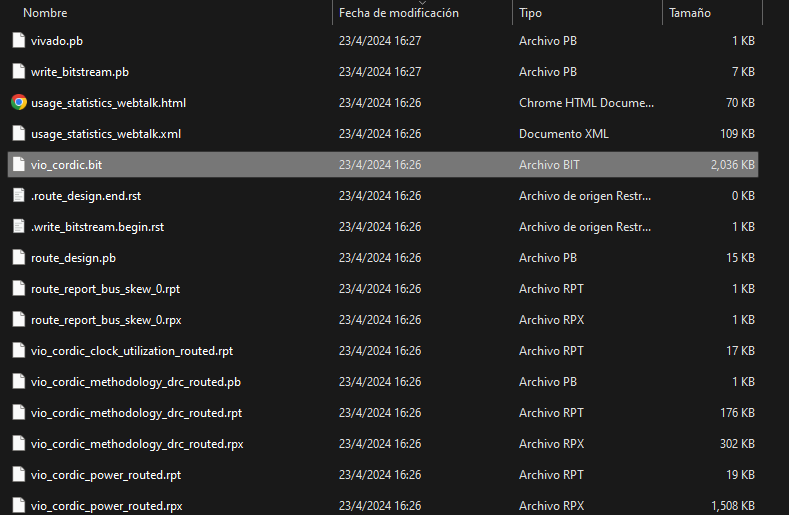
\includegraphics[width=0.65\textwidth]{./Figuras/archivo_bit.png}
    \caption{Archivo bit}
    \label{fig:archivo_bit}
\end{figure}


Con estos pasos, se completa tanto la simulación del diseño en Vivado como la generación del archivo .bit para programar la FPGA.

\textbf{Nota:} El trabajo desarrollado se realizó sobre una FPGA de la firma Xilinx. La placa de desarrollo utilizada es la Arty Z7-10 de la empresa Digilent.

\newpage

\section{Análisis de la Síntesis en Vivado}

El proceso de síntesis en Vivado proporciona información valiosa sobre el diseño y optimización del circuito. A continuación se presenta un análisis detallado del informe de síntesis generado:

\begin{lstlisting}[basicstyle=\small\ttfamily]
****** Vivado v2018.1 (64-bit)
  **** SW Build 2188600 on Wed Apr  4 18:40:38 MDT 2018
  **** IP Build 2185939 on Wed Apr  4 20:55:05 MDT 2018
    ** Copyright 1986-2018 Xilinx, Inc. All Rights Reserved.

...
\end{lstlisting}

El informe de síntesis proporciona información sobre la utilización de recursos, optimizaciones aplicadas, advertencias y errores encontrados durante el proceso de síntesis. A continuación se presenta un resumen de los aspectos más importantes del informe:

\begin{enumerate}
    \item El diseño fue sintetizado sin errores críticos ni advertencias críticas.
    \item Se utilizaron un total de 80 DSPs y 120 bloques de memoria BRAM.
    \item Se identificaron y eliminaron elementos de Unisim que no eran necesarios para la síntesis.
    \item Se observaron algunas advertencias relacionadas con la optimización y el uso de elementos secuenciales no utilizados.
\end{enumerate}

Este informe proporciona una visión general del proceso de síntesis y las áreas que podrían requerir atención adicional para mejorar el diseño. Es importante revisar cada sección del informe cuidadosamente para garantizar un diseño óptimo y libre de errores.

\newpage

\section{Conclusiones}

El diseño del Cordic se realizó de manera exitosa, utilizando un ancho de bits adecuado para los datos de entrada y salida, así como para los vectores $X$ e $Y$. Se implementó una tabla de valores atan para mejorar la eficiencia del algoritmo. Sin embargo, a pesar de los intentos de generar valores negativos para las coordenadas $X$ e $Y$, se observó que estas se desbordaban debido a la configuración de los cuadrantes y el ángulo de rotación. Por lo tanto, no fue posible disponer de valores de seno y coseno en el rango de coordenadas negativas.

\begin{lstlisting}[language=Verilog]

module cordic_rotator #(parameter c_parameter = 16)
                      (input clock,
                       input signed [31:0] angle,
                       input signed [c_parameter-1:0] Xin,
                       input signed [c_parameter-1:0] Yin,
                       output signed [c_parameter:0] Xout,
                       output signed [c_parameter:0] Yout);

endmodule
\end{lstlisting}


El módulo VIO se diseñó para facilitar la verificación y depuración del sistema. Proporciona entradas y salidas virtuales para simular el comportamiento del diseño en un entorno controlado. Se utilizó un ancho de bits suficiente para los datos de entrada y salida del VIO. Esto permite una fácil observación de los valores de entrada y salida durante la simulación.


El Cordic y el VIO se unificaron para formar un proyecto completo. El Cordic se utiliza para el cálculo de funciones trigonométricas, mientras que el VIO proporciona una interfaz para ingresar los datos de entrada y visualizar los resultados de salida. Esta integración permite una verificación exhaustiva del diseño y garantiza su funcionalidad correcta.

\newpage
\section{Bibliografía}

\begin{thebibliography}{6}
\bibitem{cordic_paper}
Smith, S. W. (1971). "Cordic Trigonometry". RADC Technical Report.

\bibitem{cordic_book}
Walther, J. S. (1971). "A unified algorithm for elementary functions". AFIPS Conference Proceedings.

\bibitem{cordic_survey}
Volder, J. E. (1959). "The Cordic Trigonometric Computing Technique". IRE Transactions on Electronic Computers.

\bibitem{verilog_book}
Palnitkar, S. (2003). "Verilog HDL: A Guide to Digital Design and Synthesis". Prentice Hall.

\bibitem{verilog_reference}
IEEE Standard for SystemVerilog. (2017). IEEE Std 1800-2017.

\bibitem{fpga_cookbook}
Vohra, D. (2015). "FPGA Prototyping by Verilog Examples: Xilinx Spartan-3 Version". Wiley-IEEE Press.

\end{thebibliography}




\end{document}
